<<<<<<< HEAD
\subsection{BÀI TẬP TRẮC NGHIỆM}

\ind{PHẦN I.} \inden{Câu trắc nghiệm nhiều phương án lựa chọn. Mỗi câu hỏi học sinh chỉ chọn một phương án.}\\
\setcounter{ex}{0}
\Opensolutionfile{ans}[ans/1D1-B1-1]

\begin{ex}%[0D6B1-1]
	Khẳng định nào sau đây là đúng?
	\choice
	{$1$ rad $=60^{\circ}$}
	{\True $1$ rad $={\left(\dfrac{180}{\pi}\right)}^{\circ}$}
	{$1$ rad $=1^{\circ}$}
	{$1$ rad $=180^{\circ}$}
	\loigiai{
		Ta có $\pi$ rad tướng ứng với $180^{\circ}$.
		Suy ra $1$ rad tương ứng với $x^{\circ}$. Vậy $x=\dfrac{180 \cdot 1}{\pi}$.
	}
\end{ex}\cham{4}

\begin{ex}%[0D6Y1-1]
	Đổi số đo của góc $108^{\circ}$ sang đơn vị radian.
	\choice
	{$\dfrac{3\pi}{2}$}
	{$\dfrac{\pi}{10}$}
	{\True $\dfrac{3\pi}{5}$}
	{$\dfrac{\pi}{4}$}
	\loigiai{
	}
\end{ex}\cham{4}


\begin{ex}%[0D6B1-1]
	Đổi số đo của góc $70^{\circ}$ sang đơn vị radian.
	\choice
	{$\dfrac{7}{18}$}
	{\True $\dfrac{7\pi}{18}$}
	{$\dfrac{70}{\pi}$}
	{$\dfrac{7}{18\pi}$}
	\loigiai{
		Áp dụng công thức $\alpha =\dfrac{a \cdot \pi}{180}$ với $\alpha $ tính bằng radian, $a$ tính bằng độ.\\
		Ta có $\alpha =\dfrac{a \cdot \pi}{180}=\dfrac{70\pi}{180}=\dfrac{7\pi}{18}$.
	}
\end{ex}\cham{4}

\begin{ex}%[0D6B1-1]
	Đổi số đo của góc $\dfrac{\pi}{12}$ rad sang đơn vị độ.
	\choice
	{$6^{\circ}$}
	{\True $15^{\circ}$}
	{$10^{\circ}$}
	{$5^{\circ}$}
	\loigiai{
		Từ công thức $\alpha =\dfrac{a \cdot \pi}{180}\Rightarrow a={\left(\dfrac{\alpha \cdot 180}{\pi}\right)}^{\circ}$ với $\alpha $ tính bằng radian, $a$ tính bằng độ.\\
		Ta có $a={\left(\dfrac{\alpha \cdot 180}{\pi}\right)}^{\circ}={\left(\dfrac{\dfrac{\pi}{12} \cdot 180}{\pi}\right)}^{\circ}=15^{\circ}$.
	}
\end{ex}\cham{4}

\begin{ex}%[0D6B1-1]
	Đổi số đo của góc $-5$ rad sang đơn vị độ, phút, giây.
	\choice
	{$-286^{\circ}$}
	{$286^{\circ}28'44''$}
	{$-286^{\circ}44'28''$}
	{\True $-286^{\circ}28'44''$}
	\loigiai{
		Ta có $a={\left(\dfrac{\alpha \cdot 180}{\pi}\right)}^{\circ}={\left(\dfrac{-5.180}{\pi}\right)}^{\circ}=-286^{\circ}28'44''.$
	}
\end{ex}\cham{5}

\begin{ex}%[0D6B1-5]
	Trên đường tròn cung có số đo $1$ rad là cung
	\choice
	{\True có độ dài bằng nửa đường kính}
	{có độ dài bằng đường kính}
	{có độ dài bằng 1}
	{tương ứng với góc ở tâm $60^{\circ}$}
	\loigiai{
		Cung có độ dài bằng bán kính (nửa đường kính) thì có số đó bằng $1$ rad.
	}
\end{ex}\cham{4}

\begin{ex}%[0D6B1-2]
	Tính độ dài $\ell $ của cung trên đường tròn có bán kính bằng $20$ cm và số đo $\dfrac{\pi}{16}.$
	\choice
	{$\ell =2{,}94$ cm}
	{$\ell =3{,}39$ cm}
	{$\ell =1{,}49$ cm}
	{\True $\ell =3{,}93$ cm}
	\loigiai{
		Áp dụng công thức $\ell =R\alpha =20 \cdot \dfrac{\pi}{16}\approx 3{,}93$ cm.
	}
\end{ex}\cham{4}

\begin{ex}%[0D6B1-2]
	Tính độ dài của cung trên đường tròn có số đo $1{,}5$ và bán kính bằng $20$ cm.
	\choice
	{$40$ cm}
	{$60$ cm}
	{\True $30$ cm}
	{$20$ cm}
	\loigiai{
		Ta có $\ell =\alpha R=1{,}5 \cdot 20=30$cm.
	}
\end{ex}\cham{4}


\begin{ex}
	\immini[thm]{Xác định số đo của góc lượng giác được biểu diễn trong hình bên.
		\choice
		{\True $405^\circ$}
		{$385^\circ$}
		{$-405^\circ$}
		{$45^\circ$}}{
		\begin{tikzpicture}[line width=1pt, >=Stealth]
			\def\bk{0.5}
			\def\dr{2.1}
			\path
			(0:0) coordinate (O)
			(0:\dr) coordinate (A)
			(45:\dr) coordinate (B)
			;
			\draw pic["\tiny$45^\circ$",draw,angle eccentricity=1.8,angle radius=0.3cm]{angle=A--O--B};
			\draw (0,0)coordinate(O)node[below left=-2pt]{$O$} ;
			\foreach \a in {0.3}{
				\draw [->, red] ($(O)+(0:\bk+\a)$) arc (0:270:{\bk+\a} and {\bk+ \a})
				($(O)+(270:\bk+\a)$) arc (270:360:{\bk+\a+0.2} and {\bk +\a}) arc (360:415:{\bk+\a} and {\bk +\a})
				;
			}
			\draw (O) -- (0:\dr)node[below]{$u$};
			\draw (O) -- (45:\dr)node[above left]{$v$};
	\end{tikzpicture}}
\loigiai{}
\end{ex}\cham{3}

\begin{ex}
	\immini[thm]{Xác định số đo của góc lượng giác được biểu diễn trong hình bên.
		\choice
		{$450^\circ$}
		{$-450^\circ$}
		{\True $810^\circ$}
		{$90^\circ$}}{
		\begin{tikzpicture}[font=\footnotesize,line join=round,line cap=round,>=stealth,scale=1,thick]
			\path
			(0,0) coordinate (O)
			(1.5,0) coordinate (u)
			(0,1.5) coordinate (v)
			;
			\draw
			(u)--(O)--(v)
			pic[draw,angle radius=0.15cm]{right angle=u--O--v};
			\draw[samples=200,->,red,thick] plot[domain=0:360*2+90](\x:0.3+\x/1000);
			\foreach \x/\y in {u/-80, v/180,O/-100}{\fill (\x) circle(0pt) ($(\x)+(\y:0.25cm)$) node{$\x$};}
	\end{tikzpicture}}
\loigiai{}
\end{ex}\cham{3}

\begin{ex}
	\immini[thm]{Xác định số đo của góc lượng giác được biểu diễn trong hình bên.
		\choice
		{$45^\circ$}
		{\True $-315^\circ$}
		{ $315^\circ$}
		{$405^\circ$}}{
		\begin{tikzpicture}[line width=1pt, >=Stealth]
			\def\bk{0.5}
			\def\dr{2.1}
			\path
			(0:0) coordinate (O)
			(0:\dr) coordinate (A)
			(45:\dr) coordinate (B)
			;
			\draw pic["\tiny$45^\circ$",draw,angle eccentricity=1.8,angle radius=0.3cm]{angle=A--O--B};
			\draw (0,0)coordinate(O)node[below left=-2pt]{$O$} ;
			\foreach \a in {0.3}{
				\draw [->, red] ($(O)+(0:\bk+\a)$) arc (0:-315:{\bk+\a} and {\bk+ \a})
				;
			}
			\draw (O) -- (0:\dr)node[below]{$u$};
			\draw (O) -- (45:\dr)node[above left]{$v$};
	\end{tikzpicture}}
\loigiai{}
\end{ex}\cham{3}

\begin{ex}
	Cho góc lượng giác $(Ou, Ov)$ có số đo là $-\dfrac{\pi}{4}$, góc lượng giác $(Ou, Ow)$ có số đo là $\dfrac{3 \pi}{4}$. Tìm số đo của các góc lượng giác $(Ov, Ow)$.
	\choice
	{$\dfrac{\pi}{2} +k2\pi$, $k \in \mathbb{Z}$}
	{$k2\pi$, $k \in \mathbb{Z}$}
	{\True $\pi +k2\pi$, $k \in \mathbb{Z}$ }
	{$k\pi$, $k \in \mathbb{Z}$}
	\loigiai{
		$(Ov, Ow)=(Ou, Ow)-(Ou, Ov)+k2\pi=\pi +k2\pi$, $k \in \mathbb{Z}.$}
\end{ex}\cham{3}
\begin{ex}%[0D6B1-4]
	\immini[thm]{Một chiếc đồng hồ, có kim chỉ giờ $OG$ chỉ số $9$ và kim phút $OP$ chỉ số $12$. Số đo các góc lượng giác $\left(OG,OP\right)$ là
		\choice
		{$-270^{\circ}+k360^{\circ},k\in \mathbb{Z}$}
		{$-90^\circ+k180^\circ,k\in \mathbb{Z}$}
		{$90^\circ+k360^\circ,k\in \mathbb{Z}$}
		{\True $270^{\circ}+k360^{\circ},k\in \mathbb{Z}$}}{
		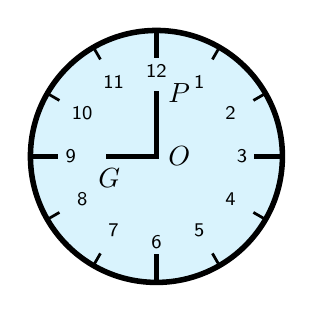
\begin{tikzpicture}[line cap=rect,line width=2pt,scale=0.8]
			\filldraw [fill=cyan!15] (0,0) circle [radius=2cm];
			\foreach \angle [count=\xi] in {60,30,...,-270}
			{
				\draw[line width=1pt] (\angle:1.8cm) -- (\angle:2cm);
				\node[font=\scriptsize] at (\angle:1.36cm) {\textsf{\xi}};
			}
			\foreach \angle in {0,90,180,270}
			\draw[line width=2pt] (\angle:1.6cm) -- (\angle:2cm);
			\draw (0,0)node[right]{$O$} -- (180:0.75cm)node[below]{$G$};
			\draw (0,0) -- (90:1cm)node[right]{$P$};
	\end{tikzpicture}}
	\loigiai{
		Theo hình vẽ, các góc lượng giác có tia đầu $OG$ và tia cuối $OP$ sẽ có số đo $-90^\circ+k360^\circ$ hay $270^{\circ}+k360^{\circ},k\in \mathbb{Z}$.
	}
\end{ex}\cham{3}

\begin{ex}%[0D6B1-3]
	Trên đường tròn lượng giác có điểm gốc là $A$. Điểm $M$ thuộc đường tròn sao cho góc lượng giác $(OA,OM)$ có số đo $45^{\circ}$. Gọi $N$ là điểm đối xứng với $M$ qua trục $Ox$. Số đo các góc lượng giác $(OA,ON)$ là
	\choice
	{$135^{\circ}+k360^\circ$}
	{$-45^{\circ}$}
	{$315^{\circ}$}
	{\True $-45^{\circ}+k360^{\circ},k\in \mathbb{Z}$}
	\loigiai{
		Vì số đo góc lượng giác $(OA,OM)$ bằng $45^{\circ}$ nên $\widehat{AOM}=45^{\circ}$, $N$ là điểm đối xứng với $M$ qua trục $Ox$ nên $\widehat{AON}=45^{\circ}$. Do đó số đo các góc lượng giác $(OA,ON)$ là $-45^{\circ}+k360^{\circ},k\in \mathbb{Z}$.
	}
\end{ex}\cham{3}

\begin{ex}%[0D6K1-3]
	Góc lượng giác nào sau đây có các điểm biểu diễn trên đường tròn lượng giác gốc $A$ tạo thành một hình vuông?
	\choice
	{$\dfrac{k2\pi}{3}$}
	{\True $\dfrac{k\pi}{2}$}
	{$\dfrac{k\pi}{3}$ }
	{$k\pi $}
	\loigiai{
		\immini[thm]{Hình vẽ tham khảo (hình vẽ bên).
			Hình vuông $CDEF$ có góc $\widehat{DCE}$ là $45^{\circ}$
			nên góc ở tâm là $90^{\circ}$ tương ứng $\dfrac{k\pi}{2}.$
		}{
			\begin{tikzpicture}[>=stealth, scale= 1.3]
				\draw[->] (-1.4,0) -- (1.4,0) node[above] {$x$};
				\draw[->] (0,-1.4) -- (0,1.4) node[left] {$y$};
				\tkzDefPoints{0/0/O, 1/0/A, 0/1/B}
				\tkzDefPointBy[rotation = center O angle 30](A) \tkzGetPoint{F}
				\tkzDefPointBy[symmetry = center O](F)\tkzGetPoint{D}
				\tkzDefPointBy[rotation = center O angle 90](F) \tkzGetPoint{C}
				\tkzDefPointBy[symmetry = center O](C)\tkzGetPoint{E}
				\tkzDefPointBy[symmetry = center O](A)\tkzGetPoint{A'}
				\tkzDefPointBy[symmetry = center O](B)\tkzGetPoint{B'}
				\tkzDrawCircle[radius](O,A)
				\tkzDrawSegments(O,D E,C E,F C,F D,C E,D)
				\tkzLabelPoints[below left](D,B')
				\tkzLabelPoints[below right](A,E)
				\tkzLabelPoints[above right](F,B,O)
				\tkzLabelPoints[above left](C,A')
			\end{tikzpicture}
		}
	}
\end{ex}\cham{4}

\begin{ex}%[0D6K1-3]
	Góc lượng giác nào sau đây có các điểm biểu diễn trên đường tròn lượng giác gốc $A$ tạo thành một tam giác đều?
	\choice
	{$\dfrac{k\pi}{3}$}
	{$k\pi $}
	{\True $\dfrac{k2\pi}{3}$}
	{$\dfrac{k\pi}{2}$}
	\loigiai{
		Tam giác đều có góc ở đỉnh là $60^{\circ}$ nên góc ở tâm là $120^{\circ}$ tương ứng $\dfrac{k2\pi}{3}$.
	}
\end{ex}\cham{5}


\begin{ex}%[0D6B2-1]
	Cho $\alpha $ thuộc góc phần tư thứ nhất của đường tròn lượng giác. Hãy chọn kết quả đúng trong các kết quả sau đây.
	\choice
	{\True $\sin \alpha >0$}
	{$\cos \alpha <0$}
	{$\tan \alpha <0$}
	{$\cot \alpha <0$}
	\loigiai{
		Do $\alpha $ thuộc góc phần tư thứ nhất $\Rightarrow \heva{& \sin \alpha >0 \\
			& \cos \alpha >0 \\
			& \tan \alpha >0 \\
			& \cot \alpha >0.} $
	} 
\end{ex}\cham{4}

\begin{ex}%[0D6B2-1]
	Cho $\alpha $ thuộc góc phần tư thứ ba của đường tròn lượng giác. Khẳng định nào sau đây là\textbf{ sai}?
	\choice
	{\True $\sin \alpha >0$}
	{$\cos \alpha <0$}
	{$\tan \alpha >0$}
	{$\cot \alpha >0$}
	\loigiai{$\alpha $ thuộc góc phần tư thứ hai $\Rightarrow \heva{& \sin \alpha <0 \\
			& \cos \alpha <0 \\
			& \tan \alpha >0 \\
			& \cot \alpha >0.}$
	} 
\end{ex}\cham{4}

\begin{ex}%[0D6B2-2]
		Cho điểm $M (x_0;y_0)$ trên đường tròn lượng giác biểu diễn cho góc lượng giác có số đo $\dfrac{26 \pi}{3}$. Khẳng định nào sau đây là đúng?
		\choice
		{$M$ thuộc góc phần tư thứ I của đường tròn lượng giác}
		{\True $M$ thuộc góc phần tư thứ II của đường tròn lượng giác}
		{$M$ thuộc góc phần tư thứ III của đường tròn lượng giác}
		{$M$ thuộc góc phần tư thứ IV của đường tròn lượng giác}
		\loigiai{
		Xét $\dfrac{26 \pi}{3}=\dfrac{2 \pi + 24 \pi}{3}=\dfrac{2\pi}{3}+8\pi$.\\
		Suy ra điểm biểu diễn của góc lượng giác $\dfrac{26 \pi}{3}$ trùng với điểm biểu diễn của góc lượng giác $\dfrac{2 \pi}{3}$. Vậy $M$ thuộc góc phần tư thứ II của đường tròn lượng giác.
	}
\end{ex}\cham{4}

\begin{ex}%[0D6B2-3]
	Với mọi $\alpha \in \mathbb{R}$ thì $\tan \left({2017\pi+\alpha}\right)$ bằng 
	\choice
	{$-\tan \alpha$}
	{$\cot \alpha$}
	{\True $\tan \alpha$}
	{$-\cot \alpha$}
	\loigiai{  Ta có $\tan \left({2017\pi+\alpha}\right)=\tan \alpha.$} 
\end{ex}\cham{5}

\begin{ex}%[0D6B2-3]
	Với mọi số thực $\alpha $, ta có $\sin \left({\dfrac{{9\pi}}{2}+\alpha}\right)$ bằng
	\choice
	{$-\sin \alpha$}
	{\True $\cos \alpha$}
	{$\sin \alpha$}
	{$-\cos \alpha$}
	\loigiai{Ta có $\sin \left({\dfrac{{9\pi}}{2}+\alpha}\right)=\sin \left({4\pi+\dfrac{\pi}{2}+\alpha}\right)=\sin \left({\dfrac{\pi}{2}+\alpha}\right)=\cos \alpha.$  } 
\end{ex}\cham{4}

\begin{ex}%[0D6B2-3]
	Biết $A,B,C$ là các góc của tam giác $ABC$, mệnh đề nào sau đây đúng.
	\choice
	{$\sin \left({A+C}\right)=-\sin B$}
	{\True $\cos \left({A+C}\right)=-\cos B$}
	{$\tan \left({A+C}\right)=\tan B$}
	{$\cot \left({A+C}\right)=\cot B$}
	\loigiai{Vì $A,B,C$ là ba góc của một tam giác suy ra $A+C=\pi-B.$\\
		Khi đó $\sin \left({A+C}\right)=\sin \left({\pi-B}\right)=\sin B;\cos \left({A+C}\right)=\cos \left({\pi-B}\right)=-\cos B.$\\
		$\tan \left({A+C}\right)=\tan \left({\pi-B}\right)=-\tan B;\cot \left({A+C}\right)=\cot \left({\pi-B}\right)=-\cot B.$
	} 
\end{ex}\cham{5}


\begin{ex}%[0D6B2-2]
	Cho góc $\alpha $ thỏa mãn $\sin \alpha =\dfrac{{12}}{{13}}$ và $\dfrac{\pi}{2}<\alpha <\pi $. Tính $\cos \alpha.$
	\choice
	{$\cos \alpha =\dfrac{1}{{13}}$}
	{$\cos \alpha =\dfrac{5}{{13}}$}
	{\True $\cos \alpha =-\dfrac{5}{{13}}$}
	{$\cos \alpha =-\dfrac{1}{{13}}$}
	\loigiai{Vì $\dfrac{\pi}{2}<\alpha <\pi $ nên $\cos \alpha <0 $. Suy ra $ \cos \alpha =- \sqrt{{1-{\sin}^2\alpha}}=- \dfrac{5}{{13}}$
	} 
\end{ex}\cham{5}

\begin{ex}%[0D6B2-2]
	Cho góc $\alpha $ thỏa mãn $\cos \alpha =-\dfrac{{\sqrt{5}}}{3}$ và $\pi <\alpha <\dfrac{{3\pi}}{2}$. Tính $\tan \alpha.$
	\choice
	{$\tan \alpha =-\dfrac{3}{{\sqrt{5}}}$}
	{\True $\tan \alpha =\dfrac{2}{{\sqrt{5}}}$}
	{$\tan \alpha =-\dfrac{4}{{\sqrt{5}}}$}
	{$\tan \alpha =-\dfrac{2}{{\sqrt{5}}}$}
	\loigiai{Vì  $\pi <\alpha <\dfrac{{3\pi}}{2}$ nên $\tan \alpha >0$. Suy ra $ \tan \alpha = \sqrt{\dfrac{1}{\cos ^2\alpha} -1}=\dfrac{2}{{\sqrt{5}}}.$
		
	} 
\end{ex}\cham{5}

\begin{ex}%[0D6K2-2]
	Cho góc $\alpha $ thỏa mãn $\tan \alpha =2.$ Tính giá trị biểu thức $P=\dfrac{{3\sin \alpha-2\cos \alpha}}{{5\cos \alpha+7\sin \alpha}}.$ 
	\choice
	{$P=-\dfrac{4}{9}$}
	{$P=\dfrac{4}{9}$}
	{$P=-\dfrac{4}{{19}}$}
	{\True $P=\dfrac{4}{{19}}$}
	\loigiai{Chia cả tử và mẫu của $P$ cho $\cos \alpha $ ta được $P=\dfrac{{3\tan \alpha-2}}{{5+7\tan \alpha}}=\dfrac{{3\cdot 2-2}}{{5+7\cdot 2}}=\dfrac{4}{{19}}.$
		
	} 
\end{ex}\cham{5}

\Closesolutionfile{ans}

\ind{PHẦN II.} \inden{Câu trắc nghiệm đúng sai. Trong mỗi ý a), b), c), d) ở mỗi câu, học sinh chọn đúng hoặc sai.}\\
\Opensolutionfile{ans}[ans/1D1-B1-2]


\begin{ex}%[1C1B1-3]
	\immini[thm]{Cho lục giác đều $A B C D E F$ nội tiếp trong đường tròn lượng giác (thứ tự đi từ $A$ đến các đỉnh theo chiều ngược chiều kim đồng hồ). Xét tính đúng sai của các khẳng định sau:
		\choiceTF
		{\True Các góc lượng giác $(OA, OB)$ có số đo là $\dfrac{\pi}{3}+k2\pi, k\in \mathbb{Z}$}
		{\True Các góc lượng giác $(OA, OC)$ có số đo là $\dfrac{2\pi}{3}+k2\pi, k\in \mathbb{Z}$}
		{ Các góc lượng giác $(OA, OE)$ có số đo là $\dfrac{2\pi}{3}+k2\pi, k\in \mathbb{Z}$}
		{ Các góc lượng giác $(OA, OF)$ có số đo là $\dfrac{\pi}{3}+k2\pi, k\in \mathbb{Z}$}
	}{
		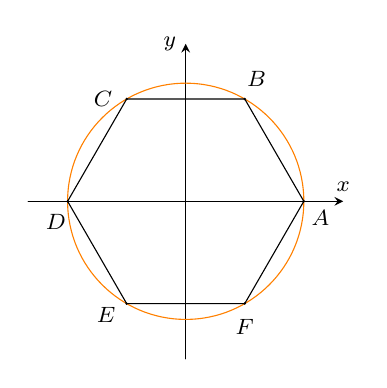
\begin{tikzpicture}[line join = round, line cap = round, >=stealth, font=\footnotesize, scale=0.5]
			\tikzset{label style/.style={font=\footnotesize}}
			\path (0,0) coordinate (O)
			(3,0) coordinate (A)
			(0:0)++(60:3) coordinate (B)
			(0:0)++(120:3) coordinate (C)
			(0:0)++(180:3) coordinate (D)
			(0:0)++(240:3) coordinate (E)
			(0:0)++(300:3) coordinate (F)
			;
			\draw[->] (-4,0) -- (4,0) node[above]{$x$};
			\draw[->] (0,-4) -- (0.,4) node[left]{$y$};
			\draw[orange] (O) circle (3cm);
			%\draw[rotate=0,->,red] (1.7,0) arc (0:220:1.7cm);
			%\draw[rotate=0,->,green!50!black] (0.6,0) arc (0:40:0.6cm);
			\draw (A)--(B)--(C)--(D)--(E)--(F)--cycle;
			%\draw (1,0) node[above,blue] {$\alpha$};
			%\draw (-1.2,1) node[below,blue,rotate=60]{$180^\circ+\alpha$};
			%\draw[red] (O)--(M');
			%\draw[green!50!black] (O)--(M);
			\foreach \p/\r in {A/-45,B/60,C/180,D/240,E/-150,F/-90}
			\fill (\p) circle (1pt) node[shift={(\r:3mm)},black]{$\p$};
	\end{tikzpicture}}
	\loigiai{
		\immini[thm]{Ta có 
			\begin{eqnarray*}
				\textrm{sđ}(OA, OB)&=& \dfrac{\pi}{3}+k2\pi, k\in \mathbb{Z}\\
				\textrm{sđ}(OA, OC)&=& \dfrac{2\pi}{3}+k2\pi, k\in \mathbb{Z}\\
					\textrm{sđ}(OA, OE)&=& -\dfrac{2\pi}{3}+k2\pi , k\in \mathbb{Z}\\
				\textrm{sđ}(OA, OF)&=& -\dfrac{\pi}{3}+k2\pi , k\in \mathbb{Z}.\\
			\end{eqnarray*}
		}{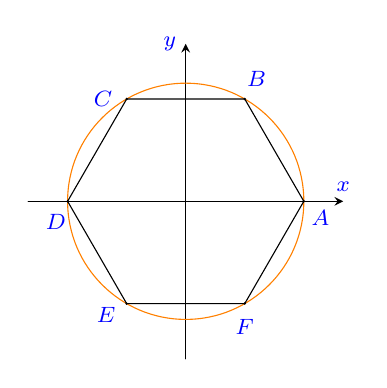
\begin{tikzpicture}[line join = round, line cap = round, >=stealth, font=\footnotesize, scale=0.5]
				\tikzset{label style/.style={font=\footnotesize}}
				\path (0,0) coordinate (O)
				(3,0) coordinate (A)
				(0:0)++(60:3) coordinate (B)
				(0:0)++(120:3) coordinate (C)
				(0:0)++(180:3) coordinate (D)
				(0:0)++(240:3) coordinate (E)
				(0:0)++(300:3) coordinate (F)
				;
				\draw[->] (-4,0) -- (4,0) node[above,blue]{$x$};
				\draw[->] (0,-4) -- (0.,4) node[left,blue]{$y$};
				\draw[orange] (O) circle (3cm);
				%\draw[rotate=0,->,red] (1.7,0) arc (0:220:1.7cm);
				%\draw[rotate=0,->,green!50!black] (0.6,0) arc (0:40:0.6cm);
				\draw (A)--(B)--(C)--(D)--(E)--(F)--cycle;
				%\draw (1,0) node[above,blue] {$\alpha$};
				%\draw (-1.2,1) node[below,blue,rotate=60]{$180^\circ+\alpha$};
				%\draw[red] (O)--(M');
				%\draw[green!50!black] (O)--(M);
				\foreach \p/\r in {A/-45,B/60,C/180,D/240,E/-150,F/-90}
				\fill (\p) circle (1pt) node[shift={(\r:3mm)},blue]{$\p$};
		\end{tikzpicture}}
	}
\end{ex}\cham{9}

\begin{ex}%[1D1B2-2]
	Cho biết $\sin \alpha=-\dfrac{1}{3}$. Xét tính đúng sai của các khẳng định sau:
	\choiceTF
	{Nếu $\alpha \in \left(\pi;\dfrac{3\pi}{2} \right)$ thì $\cos \alpha=\dfrac{2 \sqrt{2}}{3}$}
	{Nếu $\alpha \in \left(-\dfrac{\pi}{2};0 \right)$ thì $\cos \alpha=-\dfrac{2 \sqrt{2}}{3}$}
	{\True Nếu $\alpha \in \left(\pi;\dfrac{3\pi}{2} \right)$ thì $\tan \alpha=\dfrac{\sqrt{2}}{4}$}
	{Nếu $\alpha \in \left(\pi;\dfrac{3\pi}{2} \right)$ thì $\tan \alpha=-\dfrac{\sqrt{2}}{4}$}
	\loigiai{
		Ta có $\cos ^2 \alpha=1-\sin ^2 \alpha=1-\left(\dfrac{1}{3}\right)^2=\dfrac{8}{9}$.
		\begin{itemchoice}
			\itemch Vì $\pi<\alpha<\dfrac{3\pi}{2}$ nên $\cos \alpha<0$. Do đó $\cos \alpha=-\dfrac{2 \sqrt{2}}{3}$.
			\itemch Vì $-\dfrac{\pi}{2}<\alpha<0$ nên $\cos \alpha>0$. Do đó $\cos \alpha=\dfrac{2 \sqrt{2}}{3}$.
			\itemch $\tan \alpha=\dfrac{\sin \alpha}{\cos \alpha}=\dfrac{-\dfrac{1}{3}}{-\dfrac{2 \sqrt{2}}{3}}=\dfrac{\sqrt{2}}{4}$.
			\itemch $\tan \alpha=\dfrac{\sin \alpha}{\cos \alpha}=\dfrac{-\dfrac{1}{3}}{-\dfrac{2 \sqrt{2}}{3}}=\dfrac{\sqrt{2}}{4}$
		\end{itemchoice}
	}
\end{ex}\cham{14}

\begin{ex}%[1D1B2-2]
	Cho biết $\cos \alpha=-0{,}8$. Xét tính đúng sai của các khẳng định sau:
	\choiceTF
	{Nếu $\alpha \in \left(\dfrac{\pi}{2};\pi \right)$ thì $\sin \alpha=0{,}36$}
	{Nếu $\alpha \in \left(\pi;\dfrac{3\pi}{2} \right)$ thì $\sin \alpha=-0{,}36$}
	{\True Nếu $\alpha \in \left(\dfrac{\pi}{2};\pi \right)$ thì $\cot \alpha=-\dfrac{4}{3}$}
	{Nếu $\alpha \in \left(\dfrac{\pi}{2};\pi \right)$ thì $\cot \alpha=\dfrac{3}{4}$}
	\loigiai{
		Ta có $\sin ^2 \alpha=1-\cos ^2 \alpha=1-(-0,8)^2=0,36$
		\begin{itemchoice}
			\itemch Vì $\dfrac{\pi}{2}<\alpha<\pi$ nên $\sin \alpha>0$. Do đó $\sin \alpha=\sqrt{0,36}=0,6$.
			\itemch Vì $\pi<\alpha<\dfrac{3 \pi}{2}$ nên $\sin \alpha<0$. Do đó $\sin \alpha=-\sqrt{0,36}=-0,6$
			\itemch Xét $\alpha \in \left(\dfrac{\pi}{2};\pi \right)$ thì $\cot \alpha=\dfrac{\cos \alpha}{\sin \alpha}=\dfrac{-0,8}{0,6}=-\dfrac{4}{3}$.
			\itemch Xét $\alpha \in \left(\dfrac{\pi}{2};\pi \right)$ thì $\cot \alpha=\dfrac{\cos \alpha}{\sin \alpha}=\dfrac{-0,8}{0,6}=-\dfrac{4}{3}$.
		\end{itemchoice}
	}
\end{ex}\cham{16}

\begin{ex}%[1D1B2-2]
	Cho điểm $M (x_0;y_0)$ trên đường tròn lượng giác biểu diễn cho góc lượng giác có số đo $\alpha$ thỏa $\cot \alpha=\dfrac{7}{3}$. Xét tính đúng sai của các khẳng định sau:
	\choiceTF
	{\True $\tan\alpha=\dfrac{3}{7}$}
	{\True $x_0$ và $y_0$ cùng dấu}
	{\True $\sin^2 \alpha=\dfrac{9}{58}$}
	{\True $\cos^2 \alpha=\dfrac{49}{58}$}
	\loigiai{
		\begin{itemchoice}
			\itemch $\tan\alpha=\dfrac{1}{\cot\alpha}=\dfrac{3}{7}$
			\itemch Do $\tan\alpha=\dfrac{3}{7}>0$ nên $\sin \alpha =y_0$ và $\cos \alpha=x_0$ cùng dấu.
			\itemch $\sin^2\alpha = \dfrac{1}{1+\cot^2 \alpha}=\dfrac{9}{58}$.
			\itemch $\cos^2\alpha = 1-\sin^2\alpha =1-\dfrac{9}{58}=\dfrac{49}{58}$.
		\end{itemchoice}
	}
\end{ex}\cham{13}

\begin{ex}%[1D1K1-5]
	Trong chặng đua nước rút, bánh xe của một vận động viên đua xe đạp quay được $30$ vòng trong $8$ giây.Biết rằng bán kính của bánh xe là $35$ cm. Chọn chiều quay của bánh xe là chiều dương. Xét van $\mathrm{V}$ của bánh xe.
	\begin{center}
		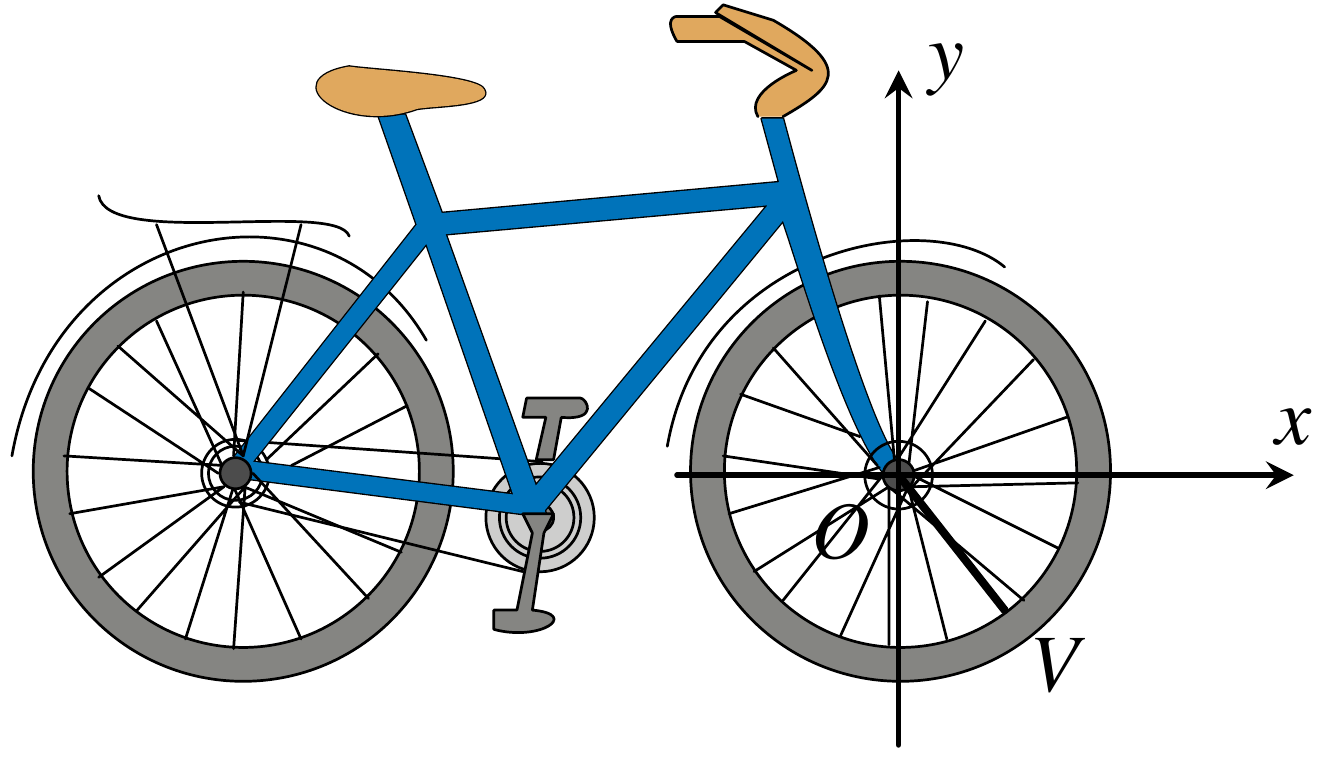
\includegraphics[scale=0.2]{images/xe-1.png}
	\end{center}
	Xét tính đúng sai của các khẳng định sau:
	\choiceTF
	{Sau $1$ giây, van $\mathrm{V}$ của bánh xe quay được 4 vòng}
	{\True Sau $1$ phút, van $\mathrm{V}$ của bánh xe quay được $225$ vòng}
	{\True Sau $1$ phút, van $\mathrm{V}$ của bánh xe quay được một góc có số đo là $450\pi$}
	{\True Độ dài quãng đường mà vận động viên đua xe đạp đã đi được trong $1$ phút là $494{,}8$ m (làm tròn đến hàng phần chục)}
	\loigiai{
		\begin{itemchoice}
			\itemch Sau $1$ giây, van $\mathrm{V}$ của bánh xe quay được $\dfrac{30}{8}=3{,}75$ (vòng).
			\itemch Sau $1$ phút, van $\mathrm{V}$ của bánh xe quay được $3{,}75 \cdot 60=225$ (vòng)
			\itemch Suy ra sau $1$ phút, van $\mathrm{V}$ của bánh xe quay được một góc có số đo là $225\cdot 2\pi=450\pi$.
			\itemch Mỗi góc ở tâm với sô đo $1$ rad chắn một cung có độ dài bằng bán kính bánh xe $r=0{,}35$ m.\\
			Do đó độ dài quãng đường mà vận động viên đua xe đạp đã đi được trong $1$ phút là $450\pi \cdot 0{,}35\approx 494{,}8$ m.
		\end{itemchoice}
	}
\end{ex}\cham{12}

\Closesolutionfile{ans}

\ind{PHẦN III.} \inden{Câu trắc nghiệm trả lời ngắn.}\\
\Opensolutionfile{ans}[ans/1D1-B1-3]

\begin{ex}%[1D1B2-2]
	Biết $\sin \alpha=\dfrac{3}{5}$ và $\dfrac{\pi}{2}<\alpha<\pi$. Tính giá trị của các biểu thức $A=\dfrac{3 \sin \alpha}{2 \cos \alpha-\tan \alpha}$ (làm tròn đến hàng phần chục).\\
	\shortans[oly]{$-2{,}1$}
	\loigiai{
		Vì $\sin \alpha=\dfrac{3}{5}$ và $\dfrac{\pi}{2}<\alpha<\pi$ nên $\cos \alpha=-\dfrac{4}{5}, \tan \alpha=-\dfrac{3}{4}$ và $\cot \alpha=-\dfrac{4}{3}$. Suy ra
		$$A=\dfrac{3 \cdot \dfrac{3}{5}}{2 \cdot\left(-\dfrac{4}{5}\right)-\left(-\dfrac{3}{4}\right)}=-\dfrac{36}{17} \approx 2,1 $$
	}
\end{ex}\cham{6}

\begin{ex}%[0D6Y1-2]%
	Một đường tròn có bán kính $30$ cm. Tìm độ dài của cung có số đo $\dfrac{\pi}{15}$ (kết quả tính bằng đơn vị cm và làm tròn đến hàng phần trăm).\\
	\shortans[oly]{$6{,}28$}
	\loigiai{
		Độ dài của cung có số đo $\dfrac{\pi}{15}$ là $l_1 = \dfrac{\pi}{15} \cdot 30 = 2 \pi \approx 6,28$ (cm).\\
	}
\end{ex}\cham{4}

\begin{ex}
	Bánh xe của người đi xe đạp quay được 15 vòng trong 8 giây. Tính độ dài quãng đường mà người đi xe đã đi được trong 2 phút, biết rằng đường kính của bánh xe đạp là 700 mm (kết quả tính bằng m và làm tròn đến hàng đơn vị).\\
	\shortans[oly]{$495$}
	\loigiai{
		\begin{enumerate}[$\bullet$]
			\item Với mỗi vòng bánh xe đã quay được một góc $360{}^\circ $ (hay $2\pi $)
			Trong 8 giây bánh xe quay được 15 vòng nên 1 giây bánh xe quay được một góc $\alpha =\dfrac{15}{8}.2\pi =\dfrac{15\pi}{4}\Rightarrow \alpha =675{}^\circ $ 
			\item Trong 1 giây bánh xe quay được một góc $\alpha =\dfrac{15\pi}{4}$ nên quãng đường mà xe đi được trong thời gian 2 phút là $l=\dfrac{15\pi}{4}.\dfrac{700}{2}.120=4948008,429mm\approx 495 m$
		\end{enumerate}
	}
\end{ex}\cham{5}

\begin{ex}%[1K1K1-8]%[Đào Trung Kiên]
	Kim giờ dài $6$ cm và kim phút dài $11$ cm của đồng hồ chỉ $4$ giờ. Hỏi thời gian ít nhất để hai kim vuông góc với nhau là bao nhiêu? Lúc đó tổng quãng đường hai đầu mút kim giờ và kim phút đi được là bao nhiêu? (kết quả được tính bằng đơn vị cm và làm tròn đến hàng phần trăm)\\
	\shortans[oly]{$6{,}57$}
	\loigiai{\begin{center}
			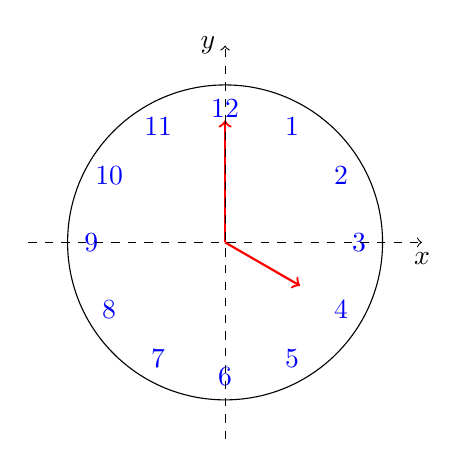
\begin{tikzpicture}
				% Vẽ đường tròn lượng giác
				\draw (0,0) circle (2cm);
				
				% Vẽ cung 2π/3
				\draw[->,red, thick] (0,0) -- ({1.55*cos(90)}, {1.55*sin(90)});
				\draw[->,red, thick] (0,0) -- ({1.1*cos(-30)}, {1.1*sin(-30)});
				\draw[blue]({1.7*cos(-30)}, {1.7*sin(-30)}) node{$4$};
				\draw[blue]({1.7*cos(0)}, {1.7*sin(0)}) node{$3$};
				\draw[blue]({1.7*cos(30)}, {1.7*sin(30)}) node{$2$};
				\draw[blue]({1.7*cos(60)}, {1.7*sin(60)}) node{$1$};
				\draw[blue]({1.7*cos(90)}, {1.7*sin(90)}) node{$12$};
				\draw[blue]({1.7*cos(120)}, {1.7*sin(120)}) node{$11$};
				\draw[blue]({1.7*cos(150)}, {1.7*sin(150)}) node{$10$};
				\draw[blue]({1.7*cos(180)}, {1.7*sin(180)}) node{$9$};
				\draw[blue]({1.7*cos(210)}, {1.7*sin(210)}) node{$8$};
				\draw[blue]({1.7*cos(240)}, {1.7*sin(240)}) node{$7$};
				\draw[blue]({1.7*cos(270)}, {1.7*sin(270)}) node{$6$};
				\draw[blue]({1.7*cos(300)}, {1.7*sin(300)}) node{$5$};
				% Ghi chú cho cung
				\draw[dashed,->] (-2.5,0) -- (2.5,0) node[below] {$x$};
				\draw[dashed,->] (0,-2.5) -- (0,2.5) node[left] {$y$};
			\end{tikzpicture}
		\end{center}
		Sau $t$ (giờ) từ lúc $4$ giờ kim phút quay tới góc $90^{\circ}-t\cdot 360^{\circ}$ và kim giờ quay tới góc $-30^{\circ}-t\cdot 30^{\circ}$.\\
		Hai kim ở vị trí vuông góc sớm nhất khi $90^{\circ}-t\cdot 360^{\circ}-(-30^{\circ}-t\cdot 30^{\circ})=90^{\circ}\Rightarrow t =\dfrac{1}{11}$.\\
		Vậy thời gian ngắn nhất để hai kim ở vị trí vuông góc là sau $\dfrac{1}{11}$ giờ.\\
		Lúc đó tổng quãng đường của hai đầu kim đi được là $$S=\dfrac{1}{11}\cdot 2\pi\cdot 11+\dfrac{1}{11}\cdot \dfrac{2\pi}{12}\cdot 6=\dfrac{23\pi}{11}\approx 6{,}57\, \text{cm}.$$
		
	}
\end{ex}\cham{5}

\begin{ex}%[1D1T2-5]
	\immini[thm]{Thanh $O M$ quay ngược chiều kim đồng hồ quanh gốc $O$ của nó trên một mặt phẳng thẳng đứng và in bóng vuông góc xuống mặt đất như hình bên. Vị trí ban đầu của thanh là $OA$. Hỏi độ dài bóng $O'M$ của $O M$ khi thanh quay được $\dfrac{60}{13}$ vòng là bao nhiêu, biết độ dài thanh $O M$ là $10 \mathrm{~cm}$? Kết quả tính theo đơn vị cm và làm tròn đến hàng phần mười.\\
		\shortans[oly]{$7{,}5$}
	}{\begin{tikzpicture}[scale=1, font=\footnotesize, line join=round, line cap=round, >=stealth]
			\def\r{1.5}
			\path
			(0:0) coordinate (O)
			(0:\r) coordinate (A)
			(200:\r) coordinate (M)
			(-2.5,-\r-0.7) coordinate (m)
			(2.5,-\r-0.7) coordinate (n)
			($(m)!(O)!(n)$) coordinate (O')
			($(m)!(M)!(n)$) coordinate (M')
			;
			\draw 
			(O)--(O') (M)--(M') (O)--(A)
			;
			\draw[thick] (m)--(n) (O)--(M);
			\draw[dashed] 
			(O) circle (\r)
			;
			\draw[thick,->] (0,\r+1.6)--(0,\r+0.6);
			\draw[thick,->] (-0.5,\r+1.6)--(-0.5,\r+0.6);
			\draw[thick,->] (0.5,\r+1.6)--(0.5,\r+0.6)node[pos=0.5,right]{ánh sáng};
			\foreach \p/\g in {O/-50, A/0, M/190, O'/-90, M'/-90}
			\draw[fill=black] (\p) circle (1pt) node[shift=(\g:3mm)] {$\p$};
			%	\pic[draw,angle radius=2mm]{angle=A--H--O};
	\end{tikzpicture}}
	\loigiai{
		Ta có $\alpha=\dfrac{60}{13} \cdot 2 \pi=\dfrac{120 \pi}{13}$.\\
		Suy ra $O'M'=\left|OM \cos \alpha\right|=\left|10 \cos \dfrac{120 \pi}{13}\right| \approx 7{,}5 \mathrm{~cm}$.
	}
\end{ex}\cham{4}

\Closesolutionfile{ans}
=======
\subsection{BÀI TẬP TRẮC NGHIỆM}

\ind{PHẦN I.} \inden{Câu trắc nghiệm nhiều phương án lựa chọn. Mỗi câu hỏi học sinh chỉ chọn một phương án.}\\
\setcounter{ex}{0}
\Opensolutionfile{ans}[ans/1D1-B1-1]

\begin{ex}%[0D6B1-1]
	Khẳng định nào sau đây là đúng?
	\choice
	{$1$ rad $=60^{\circ}$}
	{\True $1$ rad $={\left(\dfrac{180}{\pi}\right)}^{\circ}$}
	{$1$ rad $=1^{\circ}$}
	{$1$ rad $=180^{\circ}$}
	\loigiai{
		Ta có $\pi$ rad tướng ứng với $180^{\circ}$.
		Suy ra $1$ rad tương ứng với $x^{\circ}$. Vậy $x=\dfrac{180 \cdot 1}{\pi}$.
	}
\end{ex}\cham{4}

\begin{ex}%[0D6Y1-1]
	Đổi số đo của góc $108^{\circ}$ sang đơn vị radian.
	\choice
	{$\dfrac{3\pi}{2}$}
	{$\dfrac{\pi}{10}$}
	{\True $\dfrac{3\pi}{5}$}
	{$\dfrac{\pi}{4}$}
	\loigiai{
	}
\end{ex}\cham{4}


\begin{ex}%[0D6B1-1]
	Đổi số đo của góc $70^{\circ}$ sang đơn vị radian.
	\choice
	{$\dfrac{7}{18}$}
	{\True $\dfrac{7\pi}{18}$}
	{$\dfrac{70}{\pi}$}
	{$\dfrac{7}{18\pi}$}
	\loigiai{
		Áp dụng công thức $\alpha =\dfrac{a \cdot \pi}{180}$ với $\alpha $ tính bằng radian, $a$ tính bằng độ.\\
		Ta có $\alpha =\dfrac{a \cdot \pi}{180}=\dfrac{70\pi}{180}=\dfrac{7\pi}{18}$.
	}
\end{ex}\cham{4}

\begin{ex}%[0D6B1-1]
	Đổi số đo của góc $\dfrac{\pi}{12}$ rad sang đơn vị độ.
	\choice
	{$6^{\circ}$}
	{\True $15^{\circ}$}
	{$10^{\circ}$}
	{$5^{\circ}$}
	\loigiai{
		Từ công thức $\alpha =\dfrac{a \cdot \pi}{180}\Rightarrow a={\left(\dfrac{\alpha \cdot 180}{\pi}\right)}^{\circ}$ với $\alpha $ tính bằng radian, $a$ tính bằng độ.\\
		Ta có $a={\left(\dfrac{\alpha \cdot 180}{\pi}\right)}^{\circ}={\left(\dfrac{\dfrac{\pi}{12} \cdot 180}{\pi}\right)}^{\circ}=15^{\circ}$.
	}
\end{ex}\cham{4}

\begin{ex}%[0D6B1-1]
	Đổi số đo của góc $-5$ rad sang đơn vị độ, phút, giây.
	\choice
	{$-286^{\circ}$}
	{$286^{\circ}28'44''$}
	{$-286^{\circ}44'28''$}
	{\True $-286^{\circ}28'44''$}
	\loigiai{
		Ta có $a={\left(\dfrac{\alpha \cdot 180}{\pi}\right)}^{\circ}={\left(\dfrac{-5.180}{\pi}\right)}^{\circ}=-286^{\circ}28'44''.$
	}
\end{ex}\cham{5}

\begin{ex}%[0D6B1-5]
	Trên đường tròn cung có số đo $1$ rad là cung
	\choice
	{\True có độ dài bằng nửa đường kính}
	{có độ dài bằng đường kính}
	{có độ dài bằng 1}
	{tương ứng với góc ở tâm $60^{\circ}$}
	\loigiai{
		Cung có độ dài bằng bán kính (nửa đường kính) thì có số đó bằng $1$ rad.
	}
\end{ex}\cham{4}

\begin{ex}%[0D6B1-2]
	Tính độ dài $\ell $ của cung trên đường tròn có bán kính bằng $20$ cm và số đo $\dfrac{\pi}{16}.$
	\choice
	{$\ell =2{,}94$ cm}
	{$\ell =3{,}39$ cm}
	{$\ell =1{,}49$ cm}
	{\True $\ell =3{,}93$ cm}
	\loigiai{
		Áp dụng công thức $\ell =R\alpha =20 \cdot \dfrac{\pi}{16}\approx 3{,}93$ cm.
	}
\end{ex}\cham{4}

\begin{ex}%[0D6B1-2]
	Tính độ dài của cung trên đường tròn có số đo $1{,}5$ và bán kính bằng $20$ cm.
	\choice
	{$40$ cm}
	{$60$ cm}
	{\True $30$ cm}
	{$20$ cm}
	\loigiai{
		Ta có $\ell =\alpha R=1{,}5 \cdot 20=30$cm.
	}
\end{ex}\cham{4}


\begin{ex}
	\immini[thm]{Xác định số đo của góc lượng giác được biểu diễn trong hình bên.
		\choice
		{\True $405^\circ$}
		{$385^\circ$}
		{$-405^\circ$}
		{$45^\circ$}}{
		\begin{tikzpicture}[line width=1pt, >=Stealth]
			\def\bk{0.5}
			\def\dr{2.1}
			\path
			(0:0) coordinate (O)
			(0:\dr) coordinate (A)
			(45:\dr) coordinate (B)
			;
			\draw pic["\tiny$45^\circ$",draw,angle eccentricity=1.8,angle radius=0.3cm]{angle=A--O--B};
			\draw (0,0)coordinate(O)node[below left=-2pt]{$O$} ;
			\foreach \a in {0.3}{
				\draw [->, red] ($(O)+(0:\bk+\a)$) arc (0:270:{\bk+\a} and {\bk+ \a})
				($(O)+(270:\bk+\a)$) arc (270:360:{\bk+\a+0.2} and {\bk +\a}) arc (360:415:{\bk+\a} and {\bk +\a})
				;
			}
			\draw (O) -- (0:\dr)node[below]{$u$};
			\draw (O) -- (45:\dr)node[above left]{$v$};
	\end{tikzpicture}}
\loigiai{}
\end{ex}\cham{3}

\begin{ex}
	\immini[thm]{Xác định số đo của góc lượng giác được biểu diễn trong hình bên.
		\choice
		{$450^\circ$}
		{$-450^\circ$}
		{\True $810^\circ$}
		{$90^\circ$}}{
		\begin{tikzpicture}[font=\footnotesize,line join=round,line cap=round,>=stealth,scale=1,thick]
			\path
			(0,0) coordinate (O)
			(1.5,0) coordinate (u)
			(0,1.5) coordinate (v)
			;
			\draw
			(u)--(O)--(v)
			pic[draw,angle radius=0.15cm]{right angle=u--O--v};
			\draw[samples=200,->,red,thick] plot[domain=0:360*2+90](\x:0.3+\x/1000);
			\foreach \x/\y in {u/-80, v/180,O/-100}{\fill (\x) circle(0pt) ($(\x)+(\y:0.25cm)$) node{$\x$};}
	\end{tikzpicture}}
\loigiai{}
\end{ex}\cham{3}

\begin{ex}
	\immini[thm]{Xác định số đo của góc lượng giác được biểu diễn trong hình bên.
		\choice
		{$45^\circ$}
		{\True $-315^\circ$}
		{ $315^\circ$}
		{$405^\circ$}}{
		\begin{tikzpicture}[line width=1pt, >=Stealth]
			\def\bk{0.5}
			\def\dr{2.1}
			\path
			(0:0) coordinate (O)
			(0:\dr) coordinate (A)
			(45:\dr) coordinate (B)
			;
			\draw pic["\tiny$45^\circ$",draw,angle eccentricity=1.8,angle radius=0.3cm]{angle=A--O--B};
			\draw (0,0)coordinate(O)node[below left=-2pt]{$O$} ;
			\foreach \a in {0.3}{
				\draw [->, red] ($(O)+(0:\bk+\a)$) arc (0:-315:{\bk+\a} and {\bk+ \a})
				;
			}
			\draw (O) -- (0:\dr)node[below]{$u$};
			\draw (O) -- (45:\dr)node[above left]{$v$};
	\end{tikzpicture}}
\loigiai{}
\end{ex}\cham{3}

\begin{ex}
	Cho góc lượng giác $(Ou, Ov)$ có số đo là $-\dfrac{\pi}{4}$, góc lượng giác $(Ou, Ow)$ có số đo là $\dfrac{3 \pi}{4}$. Tìm số đo của các góc lượng giác $(Ov, Ow)$.
	\choice
	{$\dfrac{\pi}{2} +k2\pi$, $k \in \mathbb{Z}$}
	{$k2\pi$, $k \in \mathbb{Z}$}
	{\True $\pi +k2\pi$, $k \in \mathbb{Z}$ }
	{$k\pi$, $k \in \mathbb{Z}$}
	\loigiai{
		$(Ov, Ow)=(Ou, Ow)-(Ou, Ov)+k2\pi=\pi +k2\pi$, $k \in \mathbb{Z}.$}
\end{ex}\cham{3}
\begin{ex}%[0D6B1-4]
	\immini[thm]{Một chiếc đồng hồ, có kim chỉ giờ $OG$ chỉ số $9$ và kim phút $OP$ chỉ số $12$. Số đo các góc lượng giác $\left(OG,OP\right)$ là
		\choice
		{$-270^{\circ}+k360^{\circ},k\in \mathbb{Z}$}
		{$-90^\circ+k180^\circ,k\in \mathbb{Z}$}
		{$90^\circ+k360^\circ,k\in \mathbb{Z}$}
		{\True $270^{\circ}+k360^{\circ},k\in \mathbb{Z}$}}{
		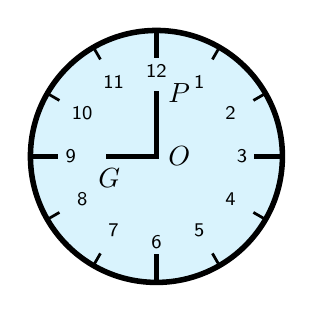
\begin{tikzpicture}[line cap=rect,line width=2pt,scale=0.8]
			\filldraw [fill=cyan!15] (0,0) circle [radius=2cm];
			\foreach \angle [count=\xi] in {60,30,...,-270}
			{
				\draw[line width=1pt] (\angle:1.8cm) -- (\angle:2cm);
				\node[font=\scriptsize] at (\angle:1.36cm) {\textsf{\xi}};
			}
			\foreach \angle in {0,90,180,270}
			\draw[line width=2pt] (\angle:1.6cm) -- (\angle:2cm);
			\draw (0,0)node[right]{$O$} -- (180:0.75cm)node[below]{$G$};
			\draw (0,0) -- (90:1cm)node[right]{$P$};
	\end{tikzpicture}}
	\loigiai{
		Theo hình vẽ, các góc lượng giác có tia đầu $OG$ và tia cuối $OP$ sẽ có số đo $-90^\circ+k360^\circ$ hay $270^{\circ}+k360^{\circ},k\in \mathbb{Z}$.
	}
\end{ex}\cham{3}

\begin{ex}%[0D6B1-3]
	Trên đường tròn lượng giác có điểm gốc là $A$. Điểm $M$ thuộc đường tròn sao cho góc lượng giác $(OA,OM)$ có số đo $45^{\circ}$. Gọi $N$ là điểm đối xứng với $M$ qua trục $Ox$. Số đo các góc lượng giác $(OA,ON)$ là
	\choice
	{$135^{\circ}+k360^\circ$}
	{$-45^{\circ}$}
	{$315^{\circ}$}
	{\True $-45^{\circ}+k360^{\circ},k\in \mathbb{Z}$}
	\loigiai{
		Vì số đo góc lượng giác $(OA,OM)$ bằng $45^{\circ}$ nên $\widehat{AOM}=45^{\circ}$, $N$ là điểm đối xứng với $M$ qua trục $Ox$ nên $\widehat{AON}=45^{\circ}$. Do đó số đo các góc lượng giác $(OA,ON)$ là $-45^{\circ}+k360^{\circ},k\in \mathbb{Z}$.
	}
\end{ex}\cham{3}

\begin{ex}%[0D6K1-3]
	Góc lượng giác nào sau đây có các điểm biểu diễn trên đường tròn lượng giác gốc $A$ tạo thành một hình vuông?
	\choice
	{$\dfrac{k2\pi}{3}$}
	{\True $\dfrac{k\pi}{2}$}
	{$\dfrac{k\pi}{3}$ }
	{$k\pi $}
	\loigiai{
		\immini[thm]{Hình vẽ tham khảo (hình vẽ bên).
			Hình vuông $CDEF$ có góc $\widehat{DCE}$ là $45^{\circ}$
			nên góc ở tâm là $90^{\circ}$ tương ứng $\dfrac{k\pi}{2}.$
		}{
			\begin{tikzpicture}[>=stealth, scale= 1.3]
				\draw[->] (-1.4,0) -- (1.4,0) node[above] {$x$};
				\draw[->] (0,-1.4) -- (0,1.4) node[left] {$y$};
				\tkzDefPoints{0/0/O, 1/0/A, 0/1/B}
				\tkzDefPointBy[rotation = center O angle 30](A) \tkzGetPoint{F}
				\tkzDefPointBy[symmetry = center O](F)\tkzGetPoint{D}
				\tkzDefPointBy[rotation = center O angle 90](F) \tkzGetPoint{C}
				\tkzDefPointBy[symmetry = center O](C)\tkzGetPoint{E}
				\tkzDefPointBy[symmetry = center O](A)\tkzGetPoint{A'}
				\tkzDefPointBy[symmetry = center O](B)\tkzGetPoint{B'}
				\tkzDrawCircle[radius](O,A)
				\tkzDrawSegments(O,D E,C E,F C,F D,C E,D)
				\tkzLabelPoints[below left](D,B')
				\tkzLabelPoints[below right](A,E)
				\tkzLabelPoints[above right](F,B,O)
				\tkzLabelPoints[above left](C,A')
			\end{tikzpicture}
		}
	}
\end{ex}\cham{4}

\begin{ex}%[0D6K1-3]
	Góc lượng giác nào sau đây có các điểm biểu diễn trên đường tròn lượng giác gốc $A$ tạo thành một tam giác đều?
	\choice
	{$\dfrac{k\pi}{3}$}
	{$k\pi $}
	{\True $\dfrac{k2\pi}{3}$}
	{$\dfrac{k\pi}{2}$}
	\loigiai{
		Tam giác đều có góc ở đỉnh là $60^{\circ}$ nên góc ở tâm là $120^{\circ}$ tương ứng $\dfrac{k2\pi}{3}$.
	}
\end{ex}\cham{5}


\begin{ex}%[0D6B2-1]
	Cho $\alpha $ thuộc góc phần tư thứ nhất của đường tròn lượng giác. Hãy chọn kết quả đúng trong các kết quả sau đây.
	\choice
	{\True $\sin \alpha >0$}
	{$\cos \alpha <0$}
	{$\tan \alpha <0$}
	{$\cot \alpha <0$}
	\loigiai{
		Do $\alpha $ thuộc góc phần tư thứ nhất $\Rightarrow \heva{& \sin \alpha >0 \\
			& \cos \alpha >0 \\
			& \tan \alpha >0 \\
			& \cot \alpha >0.} $
	} 
\end{ex}\cham{4}

\begin{ex}%[0D6B2-1]
	Cho $\alpha $ thuộc góc phần tư thứ ba của đường tròn lượng giác. Khẳng định nào sau đây là\textbf{ sai}?
	\choice
	{\True $\sin \alpha >0$}
	{$\cos \alpha <0$}
	{$\tan \alpha >0$}
	{$\cot \alpha >0$}
	\loigiai{$\alpha $ thuộc góc phần tư thứ hai $\Rightarrow \heva{& \sin \alpha <0 \\
			& \cos \alpha <0 \\
			& \tan \alpha >0 \\
			& \cot \alpha >0.}$
	} 
\end{ex}\cham{4}

\begin{ex}%[0D6B2-2]
		Cho điểm $M (x_0;y_0)$ trên đường tròn lượng giác biểu diễn cho góc lượng giác có số đo $\dfrac{26 \pi}{3}$. Khẳng định nào sau đây là đúng?
		\choice
		{$M$ thuộc góc phần tư thứ I của đường tròn lượng giác}
		{\True $M$ thuộc góc phần tư thứ II của đường tròn lượng giác}
		{$M$ thuộc góc phần tư thứ III của đường tròn lượng giác}
		{$M$ thuộc góc phần tư thứ IV của đường tròn lượng giác}
		\loigiai{
		Xét $\dfrac{26 \pi}{3}=\dfrac{2 \pi + 24 \pi}{3}=\dfrac{2\pi}{3}+8\pi$.\\
		Suy ra điểm biểu diễn của góc lượng giác $\dfrac{26 \pi}{3}$ trùng với điểm biểu diễn của góc lượng giác $\dfrac{2 \pi}{3}$. Vậy $M$ thuộc góc phần tư thứ II của đường tròn lượng giác.
	}
\end{ex}\cham{4}

\begin{ex}%[0D6B2-3]
	Với mọi $\alpha \in \mathbb{R}$ thì $\tan \left({2017\pi+\alpha}\right)$ bằng 
	\choice
	{$-\tan \alpha$}
	{$\cot \alpha$}
	{\True $\tan \alpha$}
	{$-\cot \alpha$}
	\loigiai{  Ta có $\tan \left({2017\pi+\alpha}\right)=\tan \alpha.$} 
\end{ex}\cham{5}

\begin{ex}%[0D6B2-3]
	Với mọi số thực $\alpha $, ta có $\sin \left({\dfrac{{9\pi}}{2}+\alpha}\right)$ bằng
	\choice
	{$-\sin \alpha$}
	{\True $\cos \alpha$}
	{$\sin \alpha$}
	{$-\cos \alpha$}
	\loigiai{Ta có $\sin \left({\dfrac{{9\pi}}{2}+\alpha}\right)=\sin \left({4\pi+\dfrac{\pi}{2}+\alpha}\right)=\sin \left({\dfrac{\pi}{2}+\alpha}\right)=\cos \alpha.$  } 
\end{ex}\cham{4}

\begin{ex}%[0D6B2-3]
	Biết $A,B,C$ là các góc của tam giác $ABC$, mệnh đề nào sau đây đúng.
	\choice
	{$\sin \left({A+C}\right)=-\sin B$}
	{\True $\cos \left({A+C}\right)=-\cos B$}
	{$\tan \left({A+C}\right)=\tan B$}
	{$\cot \left({A+C}\right)=\cot B$}
	\loigiai{Vì $A,B,C$ là ba góc của một tam giác suy ra $A+C=\pi-B.$\\
		Khi đó $\sin \left({A+C}\right)=\sin \left({\pi-B}\right)=\sin B;\cos \left({A+C}\right)=\cos \left({\pi-B}\right)=-\cos B.$\\
		$\tan \left({A+C}\right)=\tan \left({\pi-B}\right)=-\tan B;\cot \left({A+C}\right)=\cot \left({\pi-B}\right)=-\cot B.$
	} 
\end{ex}\cham{5}


\begin{ex}%[0D6B2-2]
	Cho góc $\alpha $ thỏa mãn $\sin \alpha =\dfrac{{12}}{{13}}$ và $\dfrac{\pi}{2}<\alpha <\pi $. Tính $\cos \alpha.$
	\choice
	{$\cos \alpha =\dfrac{1}{{13}}$}
	{$\cos \alpha =\dfrac{5}{{13}}$}
	{\True $\cos \alpha =-\dfrac{5}{{13}}$}
	{$\cos \alpha =-\dfrac{1}{{13}}$}
	\loigiai{Vì $\dfrac{\pi}{2}<\alpha <\pi $ nên $\cos \alpha <0 $. Suy ra $ \cos \alpha =- \sqrt{{1-{\sin}^2\alpha}}=- \dfrac{5}{{13}}$
	} 
\end{ex}\cham{5}

\begin{ex}%[0D6B2-2]
	Cho góc $\alpha $ thỏa mãn $\cos \alpha =-\dfrac{{\sqrt{5}}}{3}$ và $\pi <\alpha <\dfrac{{3\pi}}{2}$. Tính $\tan \alpha.$
	\choice
	{$\tan \alpha =-\dfrac{3}{{\sqrt{5}}}$}
	{\True $\tan \alpha =\dfrac{2}{{\sqrt{5}}}$}
	{$\tan \alpha =-\dfrac{4}{{\sqrt{5}}}$}
	{$\tan \alpha =-\dfrac{2}{{\sqrt{5}}}$}
	\loigiai{Vì  $\pi <\alpha <\dfrac{{3\pi}}{2}$ nên $\tan \alpha >0$. Suy ra $ \tan \alpha = \sqrt{\dfrac{1}{\cos ^2\alpha} -1}=\dfrac{2}{{\sqrt{5}}}.$
		
	} 
\end{ex}\cham{5}

\begin{ex}%[0D6K2-2]
	Cho góc $\alpha $ thỏa mãn $\tan \alpha =2.$ Tính giá trị biểu thức $P=\dfrac{{3\sin \alpha-2\cos \alpha}}{{5\cos \alpha+7\sin \alpha}}.$ 
	\choice
	{$P=-\dfrac{4}{9}$}
	{$P=\dfrac{4}{9}$}
	{$P=-\dfrac{4}{{19}}$}
	{\True $P=\dfrac{4}{{19}}$}
	\loigiai{Chia cả tử và mẫu của $P$ cho $\cos \alpha $ ta được $P=\dfrac{{3\tan \alpha-2}}{{5+7\tan \alpha}}=\dfrac{{3\cdot 2-2}}{{5+7\cdot 2}}=\dfrac{4}{{19}}.$
		
	} 
\end{ex}\cham{5}

\Closesolutionfile{ans}

\ind{PHẦN II.} \inden{Câu trắc nghiệm đúng sai. Trong mỗi ý a), b), c), d) ở mỗi câu, học sinh chọn đúng hoặc sai.}\\
\Opensolutionfile{ans}[ans/1D1-B1-2]


\begin{ex}%[1C1B1-3]
	\immini[thm]{Cho lục giác đều $A B C D E F$ nội tiếp trong đường tròn lượng giác (thứ tự đi từ $A$ đến các đỉnh theo chiều ngược chiều kim đồng hồ). Xét tính đúng sai của các khẳng định sau:
		\choiceTF
		{\True Các góc lượng giác $(OA, OB)$ có số đo là $\dfrac{\pi}{3}+k2\pi, k\in \mathbb{Z}$}
		{\True Các góc lượng giác $(OA, OC)$ có số đo là $\dfrac{2\pi}{3}+k2\pi, k\in \mathbb{Z}$}
		{ Các góc lượng giác $(OA, OE)$ có số đo là $\dfrac{2\pi}{3}+k2\pi, k\in \mathbb{Z}$}
		{ Các góc lượng giác $(OA, OF)$ có số đo là $\dfrac{\pi}{3}+k2\pi, k\in \mathbb{Z}$}
	}{
		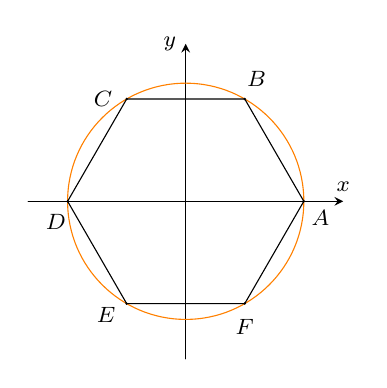
\begin{tikzpicture}[line join = round, line cap = round, >=stealth, font=\footnotesize, scale=0.5]
			\tikzset{label style/.style={font=\footnotesize}}
			\path (0,0) coordinate (O)
			(3,0) coordinate (A)
			(0:0)++(60:3) coordinate (B)
			(0:0)++(120:3) coordinate (C)
			(0:0)++(180:3) coordinate (D)
			(0:0)++(240:3) coordinate (E)
			(0:0)++(300:3) coordinate (F)
			;
			\draw[->] (-4,0) -- (4,0) node[above]{$x$};
			\draw[->] (0,-4) -- (0.,4) node[left]{$y$};
			\draw[orange] (O) circle (3cm);
			%\draw[rotate=0,->,red] (1.7,0) arc (0:220:1.7cm);
			%\draw[rotate=0,->,green!50!black] (0.6,0) arc (0:40:0.6cm);
			\draw (A)--(B)--(C)--(D)--(E)--(F)--cycle;
			%\draw (1,0) node[above,blue] {$\alpha$};
			%\draw (-1.2,1) node[below,blue,rotate=60]{$180^\circ+\alpha$};
			%\draw[red] (O)--(M');
			%\draw[green!50!black] (O)--(M);
			\foreach \p/\r in {A/-45,B/60,C/180,D/240,E/-150,F/-90}
			\fill (\p) circle (1pt) node[shift={(\r:3mm)},black]{$\p$};
	\end{tikzpicture}}
	\loigiai{
		\immini[thm]{Ta có 
			\begin{eqnarray*}
				\textrm{sđ}(OA, OB)&=& \dfrac{\pi}{3}+k2\pi, k\in \mathbb{Z}\\
				\textrm{sđ}(OA, OC)&=& \dfrac{2\pi}{3}+k2\pi, k\in \mathbb{Z}\\
					\textrm{sđ}(OA, OE)&=& -\dfrac{2\pi}{3}+k2\pi , k\in \mathbb{Z}\\
				\textrm{sđ}(OA, OF)&=& -\dfrac{\pi}{3}+k2\pi , k\in \mathbb{Z}.\\
			\end{eqnarray*}
		}{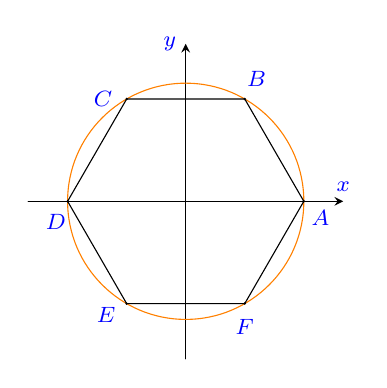
\begin{tikzpicture}[line join = round, line cap = round, >=stealth, font=\footnotesize, scale=0.5]
				\tikzset{label style/.style={font=\footnotesize}}
				\path (0,0) coordinate (O)
				(3,0) coordinate (A)
				(0:0)++(60:3) coordinate (B)
				(0:0)++(120:3) coordinate (C)
				(0:0)++(180:3) coordinate (D)
				(0:0)++(240:3) coordinate (E)
				(0:0)++(300:3) coordinate (F)
				;
				\draw[->] (-4,0) -- (4,0) node[above,blue]{$x$};
				\draw[->] (0,-4) -- (0.,4) node[left,blue]{$y$};
				\draw[orange] (O) circle (3cm);
				%\draw[rotate=0,->,red] (1.7,0) arc (0:220:1.7cm);
				%\draw[rotate=0,->,green!50!black] (0.6,0) arc (0:40:0.6cm);
				\draw (A)--(B)--(C)--(D)--(E)--(F)--cycle;
				%\draw (1,0) node[above,blue] {$\alpha$};
				%\draw (-1.2,1) node[below,blue,rotate=60]{$180^\circ+\alpha$};
				%\draw[red] (O)--(M');
				%\draw[green!50!black] (O)--(M);
				\foreach \p/\r in {A/-45,B/60,C/180,D/240,E/-150,F/-90}
				\fill (\p) circle (1pt) node[shift={(\r:3mm)},blue]{$\p$};
		\end{tikzpicture}}
	}
\end{ex}\cham{9}

\begin{ex}%[1D1B2-2]
	Cho biết $\sin \alpha=-\dfrac{1}{3}$. Xét tính đúng sai của các khẳng định sau:
	\choiceTF
	{Nếu $\alpha \in \left(\pi;\dfrac{3\pi}{2} \right)$ thì $\cos \alpha=\dfrac{2 \sqrt{2}}{3}$}
	{Nếu $\alpha \in \left(-\dfrac{\pi}{2};0 \right)$ thì $\cos \alpha=-\dfrac{2 \sqrt{2}}{3}$}
	{\True Nếu $\alpha \in \left(\pi;\dfrac{3\pi}{2} \right)$ thì $\tan \alpha=\dfrac{\sqrt{2}}{4}$}
	{Nếu $\alpha \in \left(\pi;\dfrac{3\pi}{2} \right)$ thì $\tan \alpha=-\dfrac{\sqrt{2}}{4}$}
	\loigiai{
		Ta có $\cos ^2 \alpha=1-\sin ^2 \alpha=1-\left(\dfrac{1}{3}\right)^2=\dfrac{8}{9}$.
		\begin{itemchoice}
			\itemch Vì $\pi<\alpha<\dfrac{3\pi}{2}$ nên $\cos \alpha<0$. Do đó $\cos \alpha=-\dfrac{2 \sqrt{2}}{3}$.
			\itemch Vì $-\dfrac{\pi}{2}<\alpha<0$ nên $\cos \alpha>0$. Do đó $\cos \alpha=\dfrac{2 \sqrt{2}}{3}$.
			\itemch $\tan \alpha=\dfrac{\sin \alpha}{\cos \alpha}=\dfrac{-\dfrac{1}{3}}{-\dfrac{2 \sqrt{2}}{3}}=\dfrac{\sqrt{2}}{4}$.
			\itemch $\tan \alpha=\dfrac{\sin \alpha}{\cos \alpha}=\dfrac{-\dfrac{1}{3}}{-\dfrac{2 \sqrt{2}}{3}}=\dfrac{\sqrt{2}}{4}$
		\end{itemchoice}
	}
\end{ex}\cham{14}

\begin{ex}%[1D1B2-2]
	Cho biết $\cos \alpha=-0{,}8$. Xét tính đúng sai của các khẳng định sau:
	\choiceTF
	{Nếu $\alpha \in \left(\dfrac{\pi}{2};\pi \right)$ thì $\sin \alpha=0{,}36$}
	{Nếu $\alpha \in \left(\pi;\dfrac{3\pi}{2} \right)$ thì $\sin \alpha=-0{,}36$}
	{\True Nếu $\alpha \in \left(\dfrac{\pi}{2};\pi \right)$ thì $\cot \alpha=-\dfrac{4}{3}$}
	{Nếu $\alpha \in \left(\dfrac{\pi}{2};\pi \right)$ thì $\cot \alpha=\dfrac{3}{4}$}
	\loigiai{
		Ta có $\sin ^2 \alpha=1-\cos ^2 \alpha=1-(-0,8)^2=0,36$
		\begin{itemchoice}
			\itemch Vì $\dfrac{\pi}{2}<\alpha<\pi$ nên $\sin \alpha>0$. Do đó $\sin \alpha=\sqrt{0,36}=0,6$.
			\itemch Vì $\pi<\alpha<\dfrac{3 \pi}{2}$ nên $\sin \alpha<0$. Do đó $\sin \alpha=-\sqrt{0,36}=-0,6$
			\itemch Xét $\alpha \in \left(\dfrac{\pi}{2};\pi \right)$ thì $\cot \alpha=\dfrac{\cos \alpha}{\sin \alpha}=\dfrac{-0,8}{0,6}=-\dfrac{4}{3}$.
			\itemch Xét $\alpha \in \left(\dfrac{\pi}{2};\pi \right)$ thì $\cot \alpha=\dfrac{\cos \alpha}{\sin \alpha}=\dfrac{-0,8}{0,6}=-\dfrac{4}{3}$.
		\end{itemchoice}
	}
\end{ex}\cham{16}

\begin{ex}%[1D1B2-2]
	Cho điểm $M (x_0;y_0)$ trên đường tròn lượng giác biểu diễn cho góc lượng giác có số đo $\alpha$ thỏa $\cot \alpha=\dfrac{7}{3}$. Xét tính đúng sai của các khẳng định sau:
	\choiceTF
	{\True $\tan\alpha=\dfrac{3}{7}$}
	{\True $x_0$ và $y_0$ cùng dấu}
	{\True $\sin^2 \alpha=\dfrac{9}{58}$}
	{\True $\cos^2 \alpha=\dfrac{49}{58}$}
	\loigiai{
		\begin{itemchoice}
			\itemch $\tan\alpha=\dfrac{1}{\cot\alpha}=\dfrac{3}{7}$
			\itemch Do $\tan\alpha=\dfrac{3}{7}>0$ nên $\sin \alpha =y_0$ và $\cos \alpha=x_0$ cùng dấu.
			\itemch $\sin^2\alpha = \dfrac{1}{1+\cot^2 \alpha}=\dfrac{9}{58}$.
			\itemch $\cos^2\alpha = 1-\sin^2\alpha =1-\dfrac{9}{58}=\dfrac{49}{58}$.
		\end{itemchoice}
	}
\end{ex}\cham{13}

\begin{ex}%[1D1K1-5]
	Trong chặng đua nước rút, bánh xe của một vận động viên đua xe đạp quay được $30$ vòng trong $8$ giây.Biết rằng bán kính của bánh xe là $35$ cm. Chọn chiều quay của bánh xe là chiều dương. Xét van $\mathrm{V}$ của bánh xe.
	\begin{center}
		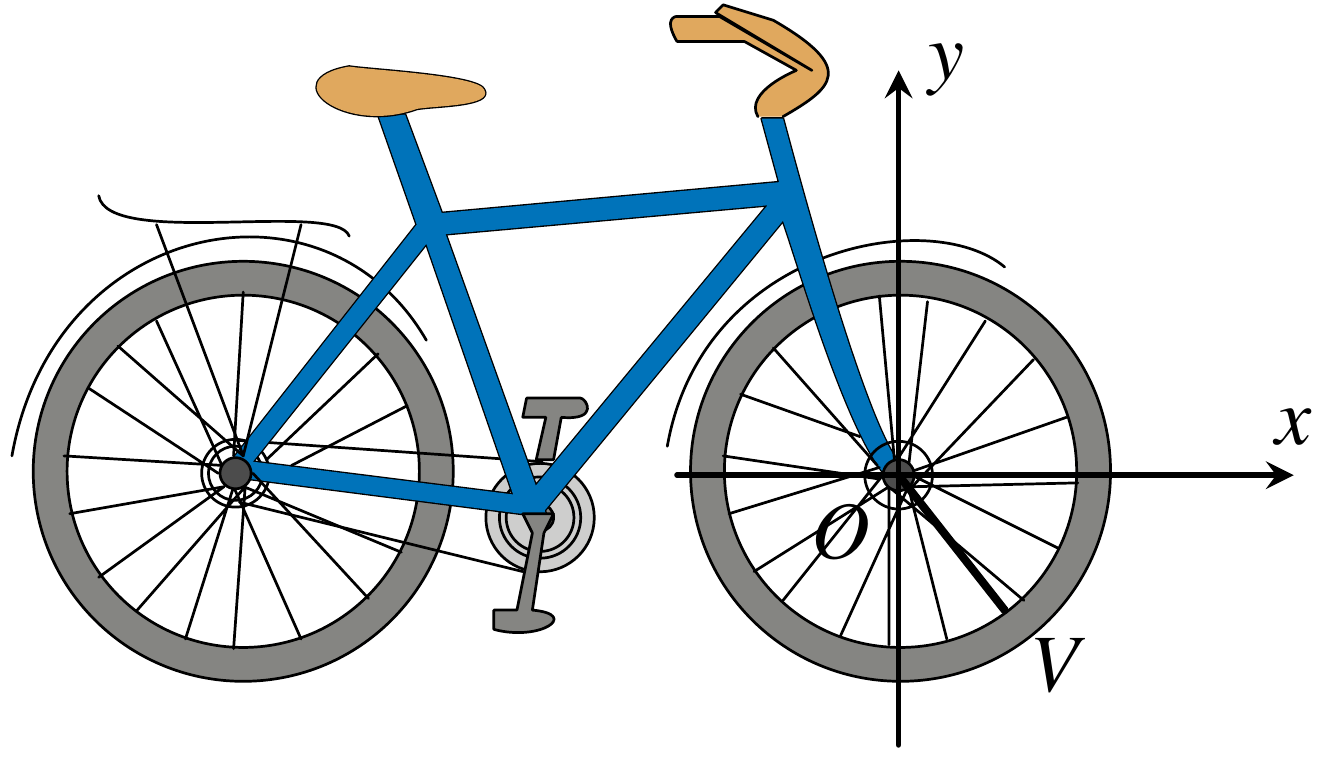
\includegraphics[scale=0.2]{images/xe-1.png}
	\end{center}
	Xét tính đúng sai của các khẳng định sau:
	\choiceTF
	{Sau $1$ giây, van $\mathrm{V}$ của bánh xe quay được 4 vòng}
	{\True Sau $1$ phút, van $\mathrm{V}$ của bánh xe quay được $225$ vòng}
	{\True Sau $1$ phút, van $\mathrm{V}$ của bánh xe quay được một góc có số đo là $450\pi$}
	{\True Độ dài quãng đường mà vận động viên đua xe đạp đã đi được trong $1$ phút là $494{,}8$ m (làm tròn đến hàng phần chục)}
	\loigiai{
		\begin{itemchoice}
			\itemch Sau $1$ giây, van $\mathrm{V}$ của bánh xe quay được $\dfrac{30}{8}=3{,}75$ (vòng).
			\itemch Sau $1$ phút, van $\mathrm{V}$ của bánh xe quay được $3{,}75 \cdot 60=225$ (vòng)
			\itemch Suy ra sau $1$ phút, van $\mathrm{V}$ của bánh xe quay được một góc có số đo là $225\cdot 2\pi=450\pi$.
			\itemch Mỗi góc ở tâm với sô đo $1$ rad chắn một cung có độ dài bằng bán kính bánh xe $r=0{,}35$ m.\\
			Do đó độ dài quãng đường mà vận động viên đua xe đạp đã đi được trong $1$ phút là $450\pi \cdot 0{,}35\approx 494{,}8$ m.
		\end{itemchoice}
	}
\end{ex}\cham{12}

\Closesolutionfile{ans}

\ind{PHẦN III.} \inden{Câu trắc nghiệm trả lời ngắn.}\\
\Opensolutionfile{ans}[ans/1D1-B1-3]

\begin{ex}%[1D1B2-2]
	Biết $\sin \alpha=\dfrac{3}{5}$ và $\dfrac{\pi}{2}<\alpha<\pi$. Tính giá trị của các biểu thức $A=\dfrac{3 \sin \alpha}{2 \cos \alpha-\tan \alpha}$ (làm tròn đến hàng phần chục).\\
	\shortans[oly]{$-2{,}1$}
	\loigiai{
		Vì $\sin \alpha=\dfrac{3}{5}$ và $\dfrac{\pi}{2}<\alpha<\pi$ nên $\cos \alpha=-\dfrac{4}{5}, \tan \alpha=-\dfrac{3}{4}$ và $\cot \alpha=-\dfrac{4}{3}$. Suy ra
		$$A=\dfrac{3 \cdot \dfrac{3}{5}}{2 \cdot\left(-\dfrac{4}{5}\right)-\left(-\dfrac{3}{4}\right)}=-\dfrac{36}{17} \approx 2,1 $$
	}
\end{ex}\cham{6}

\begin{ex}%[0D6Y1-2]%
	Một đường tròn có bán kính $30$ cm. Tìm độ dài của cung có số đo $\dfrac{\pi}{15}$ (kết quả tính bằng đơn vị cm và làm tròn đến hàng phần trăm).\\
	\shortans[oly]{$6{,}28$}
	\loigiai{
		Độ dài của cung có số đo $\dfrac{\pi}{15}$ là $l_1 = \dfrac{\pi}{15} \cdot 30 = 2 \pi \approx 6,28$ (cm).\\
	}
\end{ex}\cham{4}

\begin{ex}
	Bánh xe của người đi xe đạp quay được 15 vòng trong 8 giây. Tính độ dài quãng đường mà người đi xe đã đi được trong 2 phút, biết rằng đường kính của bánh xe đạp là 700 mm (kết quả tính bằng m và làm tròn đến hàng đơn vị).\\
	\shortans[oly]{$495$}
	\loigiai{
		\begin{enumerate}[$\bullet$]
			\item Với mỗi vòng bánh xe đã quay được một góc $360{}^\circ $ (hay $2\pi $)
			Trong 8 giây bánh xe quay được 15 vòng nên 1 giây bánh xe quay được một góc $\alpha =\dfrac{15}{8}.2\pi =\dfrac{15\pi}{4}\Rightarrow \alpha =675{}^\circ $ 
			\item Trong 1 giây bánh xe quay được một góc $\alpha =\dfrac{15\pi}{4}$ nên quãng đường mà xe đi được trong thời gian 2 phút là $l=\dfrac{15\pi}{4}.\dfrac{700}{2}.120=4948008,429mm\approx 495 m$
		\end{enumerate}
	}
\end{ex}\cham{5}

\begin{ex}%[1K1K1-8]%[Đào Trung Kiên]
	Kim giờ dài $6$ cm và kim phút dài $11$ cm của đồng hồ chỉ $4$ giờ. Hỏi thời gian ít nhất để hai kim vuông góc với nhau là bao nhiêu? Lúc đó tổng quãng đường hai đầu mút kim giờ và kim phút đi được là bao nhiêu? (kết quả được tính bằng đơn vị cm và làm tròn đến hàng phần trăm)\\
	\shortans[oly]{$6{,}57$}
	\loigiai{\begin{center}
			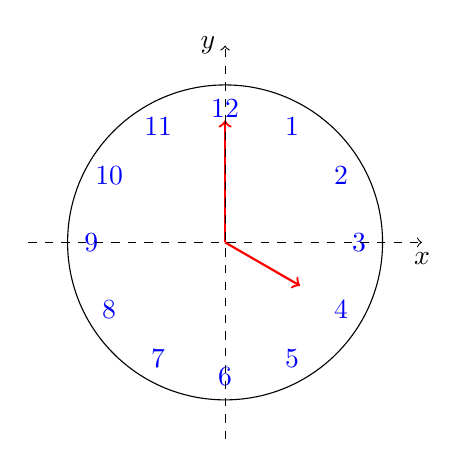
\begin{tikzpicture}
				% Vẽ đường tròn lượng giác
				\draw (0,0) circle (2cm);
				
				% Vẽ cung 2π/3
				\draw[->,red, thick] (0,0) -- ({1.55*cos(90)}, {1.55*sin(90)});
				\draw[->,red, thick] (0,0) -- ({1.1*cos(-30)}, {1.1*sin(-30)});
				\draw[blue]({1.7*cos(-30)}, {1.7*sin(-30)}) node{$4$};
				\draw[blue]({1.7*cos(0)}, {1.7*sin(0)}) node{$3$};
				\draw[blue]({1.7*cos(30)}, {1.7*sin(30)}) node{$2$};
				\draw[blue]({1.7*cos(60)}, {1.7*sin(60)}) node{$1$};
				\draw[blue]({1.7*cos(90)}, {1.7*sin(90)}) node{$12$};
				\draw[blue]({1.7*cos(120)}, {1.7*sin(120)}) node{$11$};
				\draw[blue]({1.7*cos(150)}, {1.7*sin(150)}) node{$10$};
				\draw[blue]({1.7*cos(180)}, {1.7*sin(180)}) node{$9$};
				\draw[blue]({1.7*cos(210)}, {1.7*sin(210)}) node{$8$};
				\draw[blue]({1.7*cos(240)}, {1.7*sin(240)}) node{$7$};
				\draw[blue]({1.7*cos(270)}, {1.7*sin(270)}) node{$6$};
				\draw[blue]({1.7*cos(300)}, {1.7*sin(300)}) node{$5$};
				% Ghi chú cho cung
				\draw[dashed,->] (-2.5,0) -- (2.5,0) node[below] {$x$};
				\draw[dashed,->] (0,-2.5) -- (0,2.5) node[left] {$y$};
			\end{tikzpicture}
		\end{center}
		Sau $t$ (giờ) từ lúc $4$ giờ kim phút quay tới góc $90^{\circ}-t\cdot 360^{\circ}$ và kim giờ quay tới góc $-30^{\circ}-t\cdot 30^{\circ}$.\\
		Hai kim ở vị trí vuông góc sớm nhất khi $90^{\circ}-t\cdot 360^{\circ}-(-30^{\circ}-t\cdot 30^{\circ})=90^{\circ}\Rightarrow t =\dfrac{1}{11}$.\\
		Vậy thời gian ngắn nhất để hai kim ở vị trí vuông góc là sau $\dfrac{1}{11}$ giờ.\\
		Lúc đó tổng quãng đường của hai đầu kim đi được là $$S=\dfrac{1}{11}\cdot 2\pi\cdot 11+\dfrac{1}{11}\cdot \dfrac{2\pi}{12}\cdot 6=\dfrac{23\pi}{11}\approx 6{,}57\, \text{cm}.$$
		
	}
\end{ex}\cham{5}

\begin{ex}%[1D1T2-5]
	\immini[thm]{Thanh $O M$ quay ngược chiều kim đồng hồ quanh gốc $O$ của nó trên một mặt phẳng thẳng đứng và in bóng vuông góc xuống mặt đất như hình bên. Vị trí ban đầu của thanh là $OA$. Hỏi độ dài bóng $O'M$ của $O M$ khi thanh quay được $\dfrac{60}{13}$ vòng là bao nhiêu, biết độ dài thanh $O M$ là $10 \mathrm{~cm}$? Kết quả tính theo đơn vị cm và làm tròn đến hàng phần mười.\\
		\shortans[oly]{$7{,}5$}
	}{\begin{tikzpicture}[scale=1, font=\footnotesize, line join=round, line cap=round, >=stealth]
			\def\r{1.5}
			\path
			(0:0) coordinate (O)
			(0:\r) coordinate (A)
			(200:\r) coordinate (M)
			(-2.5,-\r-0.7) coordinate (m)
			(2.5,-\r-0.7) coordinate (n)
			($(m)!(O)!(n)$) coordinate (O')
			($(m)!(M)!(n)$) coordinate (M')
			;
			\draw 
			(O)--(O') (M)--(M') (O)--(A)
			;
			\draw[thick] (m)--(n) (O)--(M);
			\draw[dashed] 
			(O) circle (\r)
			;
			\draw[thick,->] (0,\r+1.6)--(0,\r+0.6);
			\draw[thick,->] (-0.5,\r+1.6)--(-0.5,\r+0.6);
			\draw[thick,->] (0.5,\r+1.6)--(0.5,\r+0.6)node[pos=0.5,right]{ánh sáng};
			\foreach \p/\g in {O/-50, A/0, M/190, O'/-90, M'/-90}
			\draw[fill=black] (\p) circle (1pt) node[shift=(\g:3mm)] {$\p$};
			%	\pic[draw,angle radius=2mm]{angle=A--H--O};
	\end{tikzpicture}}
	\loigiai{
		Ta có $\alpha=\dfrac{60}{13} \cdot 2 \pi=\dfrac{120 \pi}{13}$.\\
		Suy ra $O'M'=\left|OM \cos \alpha\right|=\left|10 \cos \dfrac{120 \pi}{13}\right| \approx 7{,}5 \mathrm{~cm}$.
	}
\end{ex}\cham{4}

\Closesolutionfile{ans}
>>>>>>> 33890a9ce1cfbd3079ed36a93e836cf3ef1fde30
